%% vim:tw=66:spell:wrap:ft=tex
\documentclass[%
        hyperref={%
                pdfauthor={Zakariyya Mughal},%
                pdfpagemode={None},pdfpagelayout={SinglePage}}%
        xcolor={x11names},%
]{beamer}
\usetheme{Warsaw}
\usecolortheme{crane}
\usepackage{textcomp}
\usepackage{fancyvrb}
\usepackage{changepage}
\usepackage{multicol}
\usepackage{wasysym}
\usepackage[T1]{fontenc}
\newenvironment{indented}{\begin{adjustwidth}{1.5em}{}}{\end{adjustwidth}}

\usepackage{tikz}
\usetikzlibrary{snakes,arrows,shapes,automata}

\title[Regex]{Reg(ular expression\(|\)exp?)}
\author{Zaki Mughal}
\institute{University of Houston:\\CougarCS}
\date{2013 Feb 28}
\begin{document}

\frame{\titlepage}

\begin{frame}
\frametitle{What is good for?}
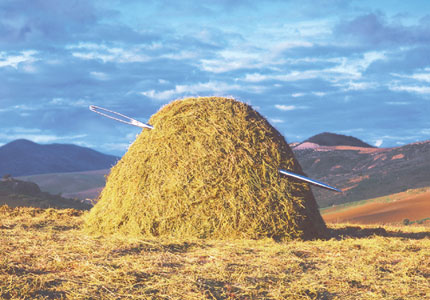
\includegraphics[width=\textwidth]{gfx/finding-a-needle-in-a-haystack.jpg}
\end{frame}

\begin{frame}
\frametitle{oblig. xkcd}
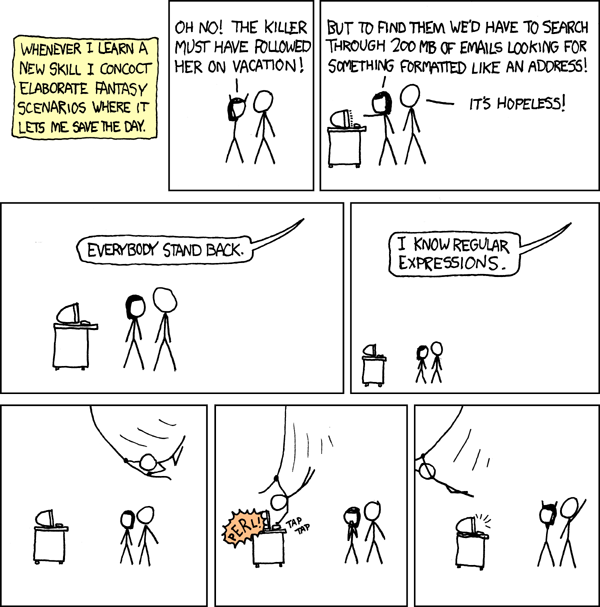
\includegraphics[height=0.90\textheight]{gfx/regular_expressions.png}
\end{frame}

\begin{frame}
\frametitle{Theory}
\begin{itemize}
	\item[] formal language theory
		\pause
	\item[] finite-state systems
	\item[] \quad neural networks (McCulloch and Pitts, 1943 !!!)
	\item[] \quad sequential circuits (Huffman\footnote{Huffman coding}, 1954 !!!)
\end{itemize}
\end{frame}

\begin{frame}
\frametitle{Finite state automata (FSA)}
\centering\resizebox{0.8\textwidth}{!}{ 
	\input{gfx/dfa.tex.in}
}

\begin{itemize}
	\item \(q_0\) is a start state (there can only be one!)
	\pause\item \(q_1\) is an accepting/final state (can be one of many)
	\pause\item follow the symbols on each path
	\pause\item all strings that end in the accepting state at end
		of the input are accepted (matched)
\end{itemize}
\pause

Matches the language that contains strings: 0, 010, 01010,
0101010, \ldots

\end{frame}

\begin{frame}
	Regular expressions are equivalent to FSA.

	Operations:
	\begin{description}
		\item [symbol] the symbol `a' matches the
			character a.
		\pause
		\item [concatenation] `ab' matches `a' followed by
			`b'
		\pause
		\item [alternation] `a+b' matches either `a' or `b'
		\pause
		\item [Kleene star] `a*' matches the empty string,
			`a', `aa', `aaa' (`a', 0 or more times)
		\pause
		\item [parentheses] can be used to group things
	\end{description}
\end{frame}

\begin{frame}
	\begin{itemize}
		\item `ab' : ab
		\pause
		\item `ab*' : a, ab, abb, abbb, abbbb, \ldots
		\pause
		\item `(ab)*' : a, ab, abab, ababab, abababab, \ldots
	\end{itemize}
\end{frame}

\begin{frame}
\frametitle{Finite state automata (FSA)}
\centering\resizebox{0.8\textwidth}{!}{ 
	\input{gfx/dfa.tex.in}
}

\begin{itemize}
	\item \(0(10)^*\)
		\pause
	\item \((01)^*0\)
		\pause
	\item \(0+(01)^*0\)
	\item[]	\quad redundant
\end{itemize}
\end{frame}

\begin{frame}
	\begin{center}
	\Huge
	We're done\ldots\newline
	\pause
	with the theory
	\end{center}
\end{frame}

\begin{frame}
	\frametitle{Regular expressions ON COMPUTERS!}
	\begin{itemize}
		\item Ken Thompson's (of Unix fame) work on text
			editors in late 60s.
		\item concatenation, parentheses, and Kleene star are the same
		\item alternation uses a pipe (\(|\)) instead of
			\(+\)
	\end{itemize}
\end{frame}

\begin{frame}
	\frametitle{Regular expressions ON COMPUTERS!}
	\begin{itemize}
		\item  ab \(\rightarrow\) ab
		\item  \((ab)^*\) \(\rightarrow\) (ab)*
		\item  a+b \(\rightarrow\) a\(|\)b
	\end{itemize}
\end{frame}

\begin{frame}
	\frametitle{Quantifiers}
	\begin{itemize}
		\item  (\(|\)a) \(\rightarrow\) a?
		\item[] \quad zero or one times: empty string or `a'
			\pause
		\item  aa* \(\rightarrow\) a+
		\item[] \quad one or more times: a, aa, aaa, \ldots
			\pause
		\item[] And just for ``fun'':
		\item  aaa+ \(\rightarrow\) a\{3,\}
		\item[] \quad 5 or more times: aaa, aaaa, aaaaa, \ldots
			\pause
		\item  (aa\(|\)aaa) \(\rightarrow\) a\{2,3\}
		\item[] \quad 2 or 3 times: aa, aaa
			\pause
		\item  aa \(\rightarrow\) a\{2\}
		\item[] \quad exactly 2 times: aa
	\end{itemize}
\end{frame}

\begin{frame}
	\frametitle{Character classes}
	\begin{itemize}
		\item $[$0123456789$]$ : any digit (0\(|\)1\(|\)2\(|\)3\(|\)4\(|\)5\(|\)6\(|\)7\(|\)8\(|\)9)
		\item $[$0-9$]$ : same thing using a range
		\item default character classes:
		\item[] \quad\quad $[[$:digit:$]]$, ($\backslash{}$d)
		\item[] \quad\quad $[[$:word:$]]$ ($\backslash{}$w)
		\item[] \quad\quad $[[$:space:$]]$ ($\backslash{}$s)
		\item any character: . (dot)
	\end{itemize}

	Match a number: $[$1-9$]$$[[$:digit:$]]$*
\end{frame}

\begin{frame}
	\frametitle{Anchors}
	\begin{itemize}
		\item \^{} (caret): beginning of line
		\item \(\$\) (dollar sign): end of line
		\item $\backslash{}$b (dollar sign): word boundary
	\end{itemize}

	Match all lines ending with spaces: $[[$:space:$]]$+\$
\end{frame}

\begin{frame}
	\frametitle{*snore*}
	\begin{itemize}
		\item it's just syntax
		\item different for different engines 
		\item \texttt{grep} (global regular expression print)
		\item \texttt{grep --color=auto}
		\item \texttt{alias grep='grep --color=auto'}
	\end{itemize}
\end{frame}

\begin{frame}
	\frametitle{Languages}
	Let's look at some different languages.

	Java, C, Perl, Python
\end{frame}

\begin{frame}
	\frametitle{Tools}
	\begin{itemize}
		\item \texttt{txt2regex} - build regex for multiple languages/tools
		\item $<$\href{http://www.regexper.com/}{http://www.regexper.com/}$>$
			: railroad diagrams
		\item $<$\href{http://www.regular-expressions.info/}{http://www.regular-expressions.info/}
		\item Friedl's ``Mastering Regular Expressions''
			from O'Reilly books
	\end{itemize}
\end{frame}

\end{document}
